\chapter{Datenverarbeitung}
\label{ch:data_processing}

\section{Klassisches Analysevorgehen}
\label{sec:common_analysis_approach_part2}

In Kapitel \ref{sec:common_analysis_approach_part1} wird beschrieben, wie bei der Open-Source Software \textit{Autopsy} ein Fall angelegt und Datenträgerabbilder hinzugefügt werden können. Schon beim Importieren einer Datenquelle können diverse Module zur automatisierten Datenaufbereitung aktiviert werden. Dies entspricht der dritten Phase, dem \textit{Sichten und Aufbereiten} aus dem allgemeinen forensischen Analyseprozess.\footnote{Siehe Abbildung \ref{fig:digital_forensics_process} in Kapitel \ref{sec:common_analysis_process}.} Diese Module werden nachfolgend beschrieben, um einen Vergleich zur hier entwickelten forensischen Analyseplattform zu ermöglichen.
Abbildung \ref{fig:autopsy_2_ingest_modules} zeigt die verfügbaren Module.

\begin{figure}[ht]
  \centering
  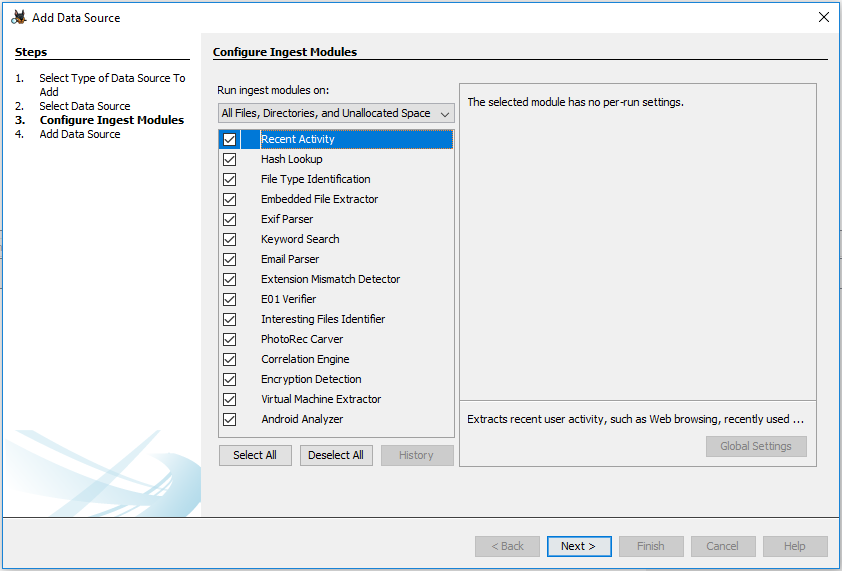
\includegraphics[width=0.78\textwidth]{./resource/autopsy_2_ingest_modules.png}
  \caption{Module zur automatischen Datenverarbeitung bei Autopsy}
  \label{fig:autopsy_2_ingest_modules}
\end{figure}

\noindent
Nachfolgend werden die Module kurz beschrieben und mit der Funktionalität der hier entwickelten forensischen Analyseplattform verglichen. Zuerst werden die Module aufgelistet, welche ganz oder teilweise in der forensischen Analyseplattform implementiert sind.\footnote{Siehe Link: \url{http://sleuthkit.org/autopsy/docs/user-docs/4.3/}. Letzter Zugriff: 09.08.2018.}

\begin{itemize}
\item Das \textit{File Type Identification Modul} ermöglicht die Ermittlung von Medientypen und Dateiformaten, wie beispielsweise \textit{JPEG}-Bilder. Autopsy nutzt hier die Open-Source Bibliothek Apache Tika\texttrademark. Eine gleichwertige Funktionalität ist auch in der forensischen Analyseplattform vorhanden.\footnote{Siehe Kapitel \ref{subsec:media_types}.}
\item Das \textit{Correlation Engine Modul} bietet eine Möglichkeit mehrere Fälle und ihre Datenquellen miteinander zu verknüpfen, um Beziehungen untereinander zu erkennen. Analog hierzu bietet auch die forensische Analyseplattform mit dem Auffinden von Datei-Duplikaten eine einfache Funktion, um Beziehungen zwischen mehreren Fällen und den Asservaten herzustellen.\footnote{Siehe Kapitel \ref{subsec:duplicate_files}.}
\item Das \textit{Keyword Search Modul} ermöglicht eine Schlüsselwortsuche. Hierzu werden Dateien mithilfe von Apache Solr indiziert. Darüber hinaus kann basierend auf regulären Ausdrücken nach bestimmten Strukturen, wie beispielsweise E-Mail- oder Web-Adressen gesucht werden. Die hier entwickelte Analyseplattform implementiert auch eine Textsuche auf Basis von Apache Solr. Derzeit ist es allerdings noch nicht möglich ganze Dateiinhalte zu indexieren.\footnote{Siehe Kapitel \ref{subsec:file_indexing}.}
\end{itemize}

\noindent
Nachfolgend werden die Module von Autopsy aufgelistet, welche noch nicht in der forensischen Analyseplattform vorhanden sind und in Weiterentwicklungen der Plattform implementiert werden könnten.
\begin{itemize}
\item Das \textit{Recent Activity Modul} versucht anhand der Zeitstempel alle interessanten Tätigkeiten der letzten 7 Tage zu ermitteln, wie zum Beispiel besuchte Websites von diversen Browsern.
\item Das \textit{Hash Lookup Modul} ermöglicht es die Datei-Hashsummen mit bereits bekannten Hashsummen zu vergleichen. Damit können bekannte Betriebssystemdateien schnell gefiltert werden. Analog zu einem Virenscanner kann dadurch auch bekannte bösartige Malware gefunden werden.
\item Das \textit{Embedded File Extractor Modul} ermöglicht das Entpacken von Archivdateien, wie beispielsweise \textit{ZIP}-Dateien.
\item Das \textit{Exif Parser Modul} ermöglicht die Anzeige der sogenannten \textit{EXIF}-Metadaten aus \textit{JPEG}-Bilddateien. In der forensischen Analyseplattform könnte diese Funktionalität auch mit Apache Tika implementiert werden.
\item Das \textit{Email Parser Modul} extrahiert E-Mails aus diversen E-Mail Archiven, wie beispielsweise dem \textit{\acrshort{pst}}-Dateiformat, welches von Microsoft Outlook genutzt wird.
\item Das \textit{Extension Mismatch Detector Modul} ermittelt Dateien, deren Dateiendung nicht zum analysierten Medientyp des Dateiinhalts passen. Dies könnte auf versteckte Dateien hinweisen. Ein ähnliche Funktion könnte in der forensischen Analyseplattform über die Volltextsuche implementiert werden, da die Dateiendung und der Medientyp bekannt sind.
\item Das \textit{E01 Verifier Modul} verifiziert speziell für das forensische Analyseformat \textit{E01} die Dateiprüfsummen mit den gespeicherten Prüfsummen. Damit können Änderungen an einem sichergestellten Asservat identifiziert werden.
\item Das \textit{Interesting Files Identifier Modul} identifiziert interessante Dateien, welche vorher durch bestimmten Suchkriterien, wie beispielsweise Dateinamen und Datentypen, definiert wurden.
\item Das \textit{PhotoRec Carver Modul} ermöglicht das bereits beschriebene File Carving auf ungenutzten Speicherbereichen. Diese Funktionalität wird nicht von der forensischen Analyseplattform unterstützt, da ungenutzte Speicherbereiche aus den originalen Datenträgerabbilder nicht in das Analysesystem importiert werden.
\item Das \textit{Encryption Detection Modul} ermöglicht das Auffinden von verschlüsselten Containern. Hierbei wird nach Dateien gesucht, deren Inhalt eine hohe Entropie aufweisen.\footnote{Die Entropie in der Informationstechnik ist ein Maß zur Bestimmung des mittleren Informationsgehalts pro Zeichen. 
%Bei verschlüsselten Containern ist diese Entropie sehr hoch verglichen zu unverschlüsselten Dateien.
}
\item Das \textit{Virtual Machine Extractor Modul} kann Dateien aus Systemabbildern von virtuellen Maschinen extrahieren.
\item Das \textit{Android Analyzer Modul} ermöglicht das Extrahieren von bestimmten Informationen aus spezifischen Dateien des Android-Betriebssystems. So können beispielsweise Kontaktdaten und Nachrichten aus spezifischen SQLite-Datenbanken ermittelt werden.
\end{itemize}

\noindent
Nachdem die benötigten Module in Autopsy aktiviert und nach fallspezifischen Eigenschaften konfiguriert wurden, erfolgt die Datenaufbereitung im Hintergrund. Parallel hierzu kann der Analyst bereits die Rohdaten analysieren.\footnote{Siehe Kapitel \ref{ch:data_visualization} zur Visualisierung von Daten.}\\

\section{Umsetzung in der forensischen Analyseplattform}

Zur Datenverarbeitung in der forensischen Analyseplattform wird Apache Spark\texttrademark\thinspace genutzt. Der physikalische Aufbau wird im Grundlagenkapitel \ref{sec:theory_spark} behandelt. In diesem Kapitel sollen primär die Algorithmen und die Verarbeitung der Daten aus logischer Sicht betrachtet.\\ 

\noindent
Bei Apache Spark (Version 2.3.0) gibt es diverse Programmierschnittstellen (\acrshort{api}s), wie Daten geladen werden können. Es besteht die Möglichkeit Daten mithilfe von \textit{\glspl{rdd}} zu laden und zu verarbeiten. Aufbauend auf diesen RDDs können die Daten konvertiert, gefiltert oder aggregiert werden.
Listing \ref{lst:spark_rdd_word_count} zeigt ein simples Beispiel zur Nutzung dieser RDDs, um alle Wörter aus einer Beispieldatei \path{history.txt} und deren Vorkommen aufzulisten. Die Implementierung kann abhängig von der Dateigröße und der Konfiguration von Spark verteilt auf mehreren Knoten ausgeführt werden, um die Datenverarbeitung zu beschleunigen. Die Daten werden aus dem HDFS gelesen und dort gespeichert.

\begin{lstlisting}[label={lst:spark_rdd_word_count},caption= Beispielimplementierung eines Spark RDDs ,captionpos=b,frame=single,style=customjava]
//Datei aus dem HDFS lesen
JavaRDD<String> textFile = sc.textFile("hdfs://data/history.txt");
JavaPairRDD<String, Integer> counts = textFile
    // Text separieren
    .flatMap(s -> Arrays.asList(s.split(" ")).iterator())
    // Wortvorkommen ermitteln
    .mapToPair(word -> new Tuple2<>(word, 1))
    .reduceByKey((a, b) -> a + b);
// Ergebnis in HDFS speichern
counts.saveAsTextFile("hdfs://...");
\end{lstlisting}


\noindent
Bei der Weiterentwicklung von Spark sind in neueren Versionen sogenannte \textit{DataFrames} und \textit{DataSets} hinzugekommen. Diese Datenstrukturen beschreiben eine Schnittstelle, welche der Sichtweise von Tabellen ähnelt. Die Implementierung dieser Typen nutzt wiederum die bereits beschriebenen RDDs.\\
Welche Datenstrukturen für die Anwendungsfälle von der forensischen Analyseplattform genutzt werden sollten, hängt primär von der Art der Daten ab.
DataFrames und DateSets sind optimiert für strukturierte und semi-strukturierte Daten. Diese Daten lassen sich beispielsweise in Tabellenstrukturen einlesen und verarbeiten. Es gibt komplexe Operationen auf diesen Tabellen, welche dem klassischen SQL Syntax sehr nahe kommen. Apache Spark kann bei der Nutzung von DataFrames und DataSets viele Optimierungen bei der Ausführung und Verarbeitung durchführen. Andererseits sind diese Strukturen ungeeignet bei unstrukturierten Daten, wie beispielsweise Multimediadateien und beliebigen Dateien im Allgemeinen.\cite[S. 66 ff.]{data_processing_spark2}\\

\noindent
Wie beim Datenimport schon beschrieben, sind die Metadaten der analysierten Datenträger strukturiert beziehungsweise semi-strukturiert in HBASE abgespeichert. Prinzipiell wäre es also möglich, auch mit DataSets und Dateframes auf diese Daten zuzugreifen. Letztlich kommt es aber auf die Anbindung zwischen Apache Spark und Apache HBASE an. Hierbei gibt es primär zwei unterschiedliche Connectoren.\footnote{Bei Apache Spark sind Connectoren eine Art von Bibliotheken, welche es ermöglichen im Ausführungskontext auf andere Systeme, wie beispielsweise Datenbanken oder Dateisysteme, zuzugreifen.} Der \textit{Hortonworks SHC} Connector ermöglicht die Interaktion mit Daten in HBASE und nutzt dafür die DataFrame/DataSet Datenstrukturen.\footnote{Siehe Link: \url{https://github.com/hortonworks-spark/shc}. Letzter Zugriff: 15.8.2018.}\\ 
Also Pendant existiert ein weiterer \textit{HBASE-Spark Connector} auf Basis von RDDs. Letzterer wird im Rahmen dieser Thesis genutzt, um Daten von HBASE zu lesen und zu schreiben.\footnote{Siehe Link: \url{https://github.com/apache/hbase/tree/master/hbase-spark} (Letzter Zugriff: 15.8.2018) und dessen Nutzung im Projekt \textit{foam-processing-spark} unter \url{https://github.com/jobusam/foam-processing-spark}, Letzter Zugriff: 25.9.2018.}
Daher wird die Datenverarbeitung mithilfe von Spark RDDs implementiert. Auch beim Auslesen von großen Dateien aus dem HDFS werden Spark RDDs verwendet, da Spark ein passende Schnittstelle zum HDFS auf Basis von RDDs anbietet.

%TODO Schreiben über getrennte Verarbeitung von großen und kleinen Dateien, da die Schnittstelle nicht einheitlich ist (siehe ByteBuffer bei HBASE und PortableDataStreams beim HDFS)

\section{Anwendungsfälle der Datenverarbeitung}
\subsection{Hashsummen ermitteln}
Eine grundlegende Funktionalität einer forensischen Analysesoftware ist die Berechnung von Hashsummen, um die Integrität fallrelevanter Dateien für zukünftige Analysen prüfen zu können. Darüber hinaus können auf Basis der Hashsummen sehr einfach Duplikate erkannt werden (siehe Kapitel \ref{subsec:duplicate_files}).\\
In der derzeitigen Implementierung wird der der \textit{\acrshort{sha}-512} Algorithmus genutzt, um eindeutige kryptografisch sichere Hashsummen zu berechnen. Bei Autopsy hingegen werden \textit{\acrshort{md5}}-Hashsummen berechnet. Der MD5-Algorithmus gilt mittlerweile jedoch als kryptografisch unsicher, da Hash-Kollisionen in wenigen Stunden berechnet werden können.\cite[S. 240-243]{hacking_and_security}\\

\noindent
Abbildung \ref{fig:data_processing_hashes} verdeutlicht den Datenfluss bei der Ermittlung von Hashsummen.
\begin{figure}[ht]
  \centering
  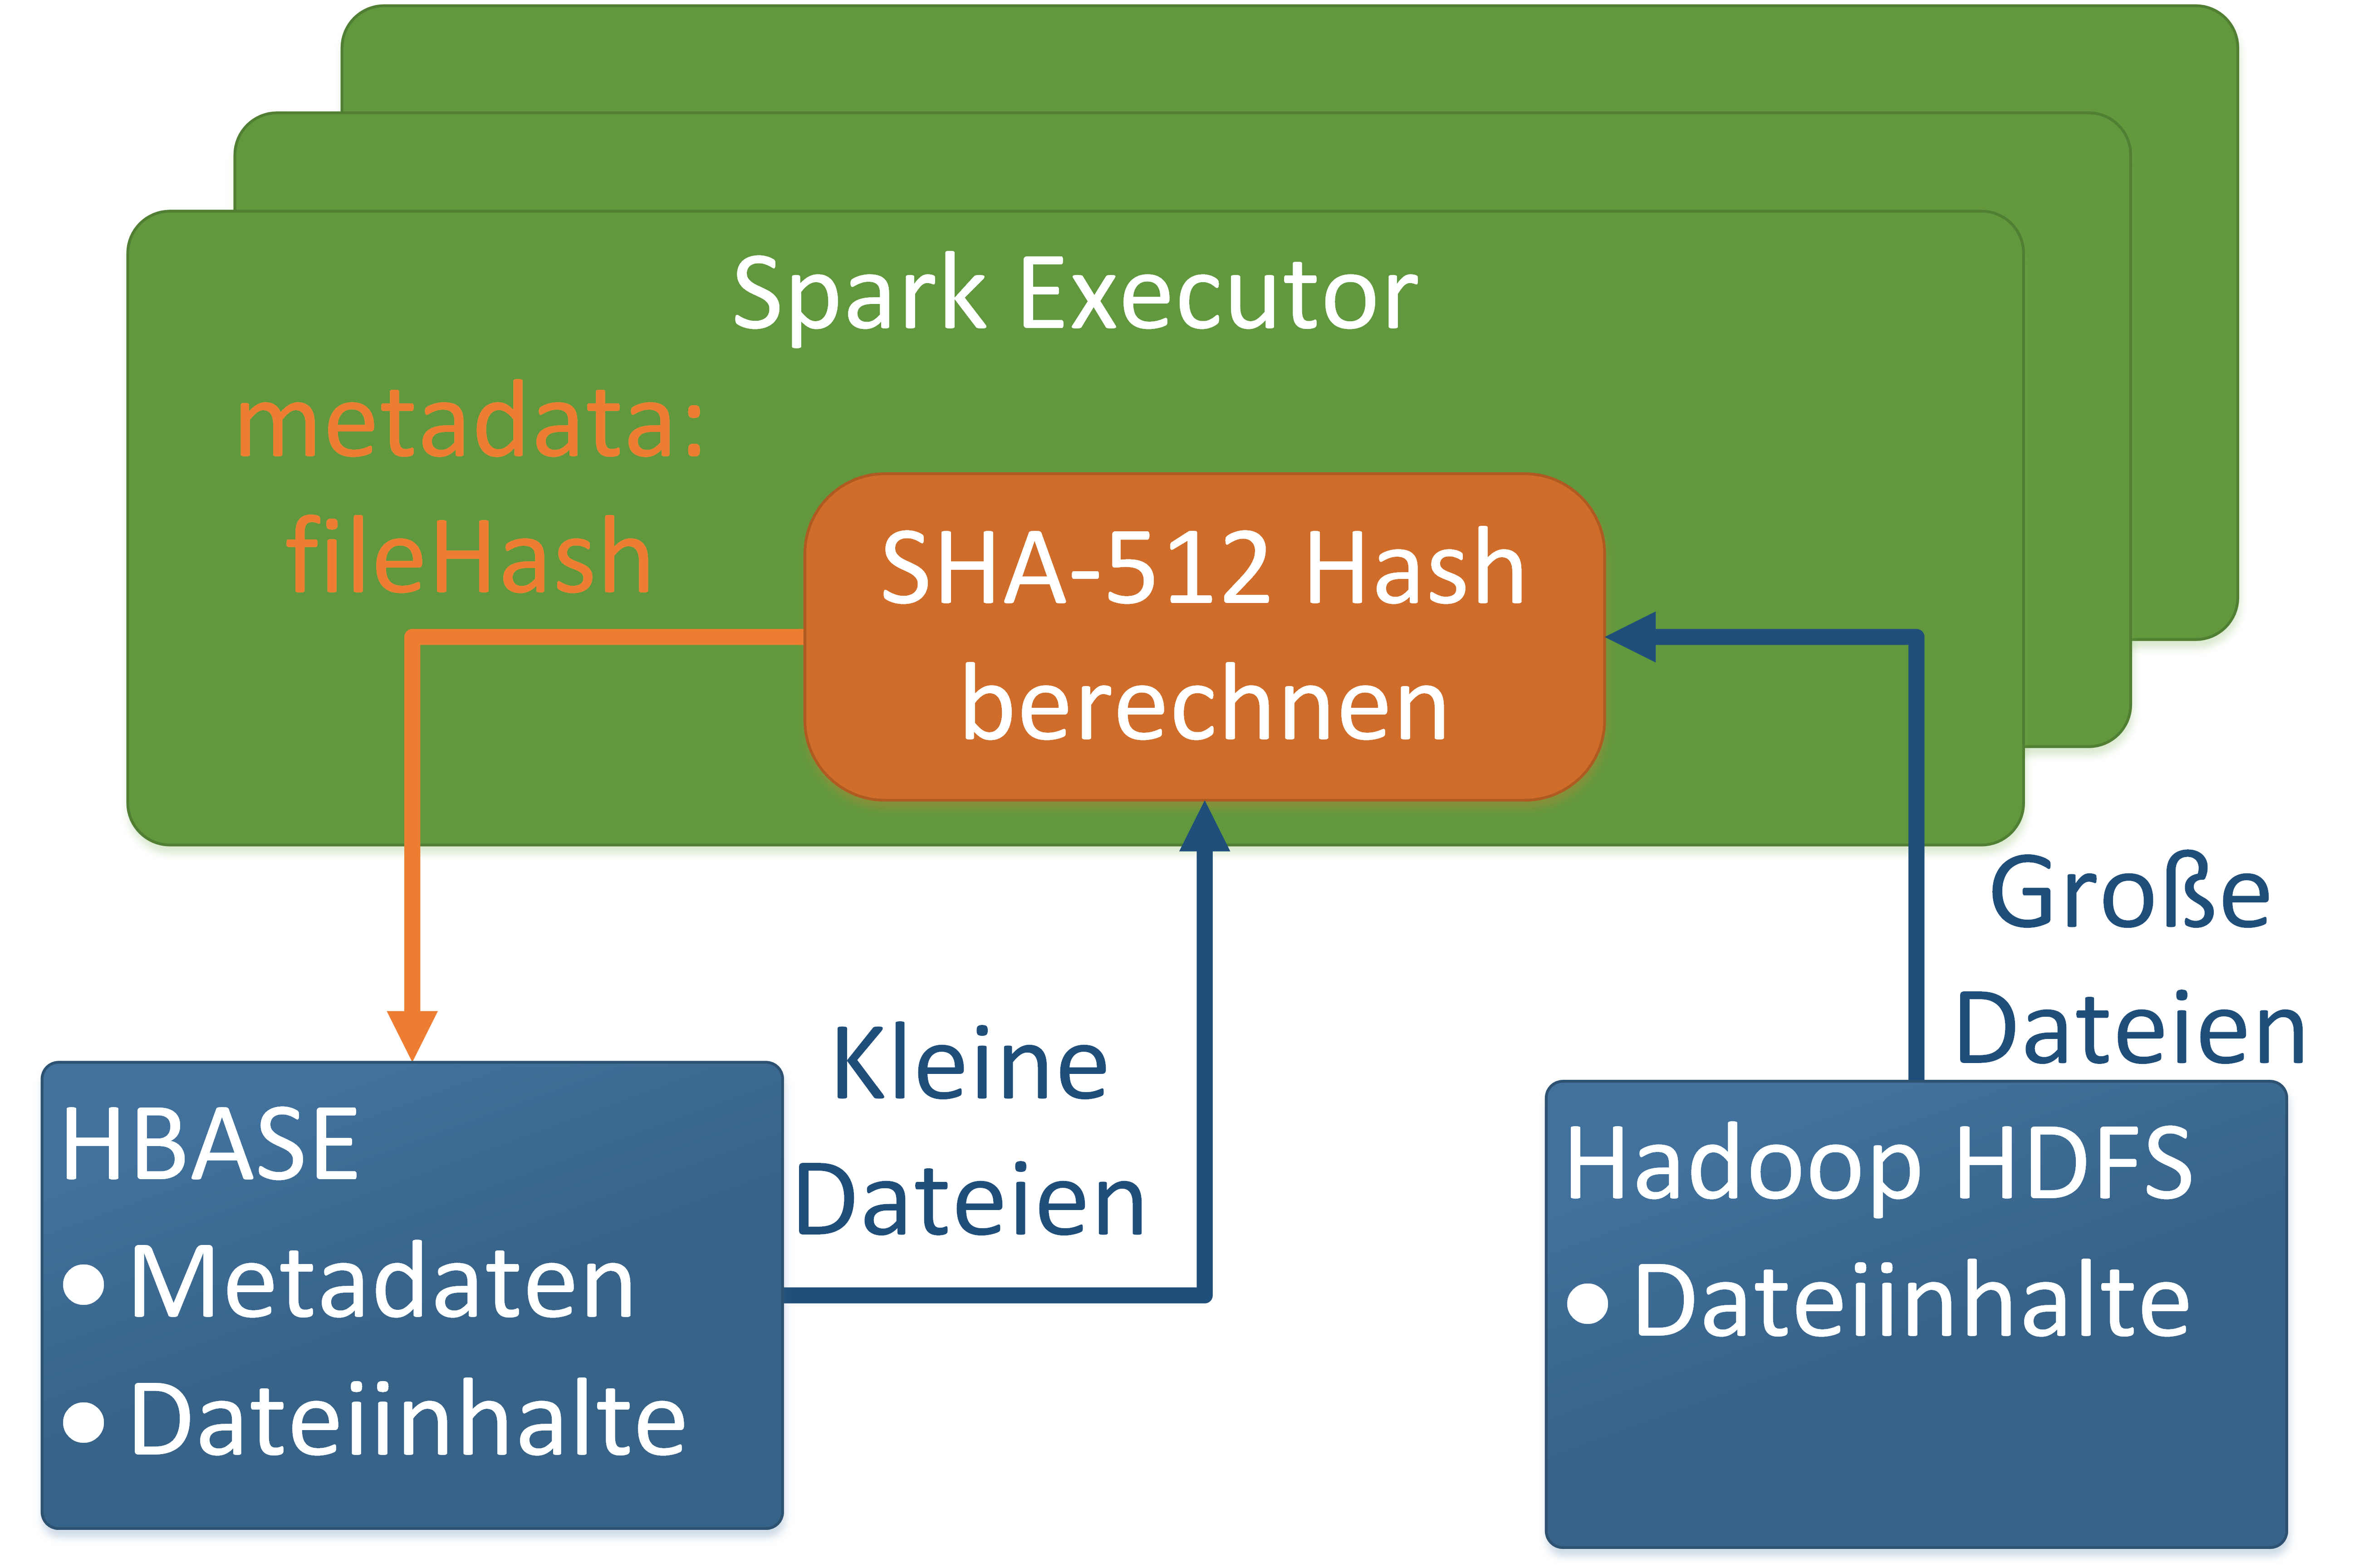
\includegraphics[width=0.78\textwidth]{./resource/spark_processing_hashes.png}
  \caption{Datenfluss bei der Berechnung von Hashsummen}
  \label{fig:data_processing_hashes}
\end{figure}

\noindent
Die Datenverarbeitung von kleinen Dateien aus HBASE und großen Dateien aus dem HDFS wird unabhängig voneinander in eigenen Spark-RDDs ausgeführt. Aufgrund der unterschiedlichen Datenquellen existieren auch zwei unterschiedliche Datentypen zum Auslesen der Dateiinhalte. Daher wird die Prozessierung in getrennten Tasks innerhalb der Spark Executoren ausgeführt. Um dann später die Hashsumme einer großen Datei aus dem HDFS in dem dazugehörigen Eintrag in HBASE abzuspeichern, ist es notwendig den Zeilenschlüssel des Eintrags in HBASE als Dateiname im HDFS zu verwenden. Dadurch können die Dateien aus dem HDFS einem Eintrag in HBASE zugeordnet werden.\\
Der ermittelte Hashwert wird darauf in der Spalte \textit{metadata:fileHash} in HBASE  gespeichert.\footnote{Siehe auch HBASE-Datenmodell in Abbildung \ref{fig:hbase_data_model}.}

\subsection{Duplikate erkennen}
\label{subsec:duplicate_files}
Aufbauend auf der Berechnung von Hashsummen können nun auch Datei-Duplikate ermittelt werden. Dadurch ist es möglich Beziehungen zwischen mehreren Asservaten herzustellen, wenn gleiche Dateien gefunden werden.\\
Derzeit werden diese Ergebnisse aber nur als Text im HDFS abgespeichert. In einer Weiterentwicklung könnten diese Informationen aber sehr gut in einer Graphendatenbank, wie beispielsweise \textit{Neo4j} abgespeichert werden. Hierdurch wäre visuell sehr schnell sichtbar, welche Beziehungen zwischen den Asservaten bestehen.\\ 
Allerdings wäre es in diesem Kontext dann auch sinnvoll, zwischen technischen Betriebssystemdateien und fachlichen Nutzerdateien zu unterscheiden. Denn wenn zwei Asservate das gleiche Betriebssystem enthalten, existieren auch zugleich tausende Datei-Duplikate. Interessant ist diese Erkennung von Duplikate aber gerade für fachliche Nutzerdaten, wie beispielsweise Bilder, Dokumente und Videos. Daran könnte später ermittelt werden, wie beispielsweise urheberrechtlich geschütztes Material über mehrere Systeme verbreitet wurde.\\

\noindent
Ein anderer Aspekt, welcher in einer Weiterentwicklung der Plattform implementiert werden könnte, ist der Vergleich mit bekannten Hashsummen von existierenden Datensätzen. Dies wird bei Autopsy verwendet, um gegebenenfalls Malware zu erkennen oder automatisiert nach spezifischen Dateien zu suchen. Ein Beispiel hierzu ist die sogenannte \textit{National Software Reference Library}, welche Hashsummen von bekannten Betriebssystem- und Anwendungsdateien enthält. Diese haben oftmals keinen forensischen Analysewert und könnten dann aus der Datenverarbeitung gefiltert werden.\footnote{Siehe Link: \url{https://www.nist.gov/itl/ssd/software-quality-group/nsrl-download/current-rds-hash-sets}. Letzter Zugriff: 9.9.2018.} \cite[S. 36]{digital_forensics}

\subsection{Medientypen erkennen}
\label{subsec:media_types}

Das Erkennen von Medientypen ist ein elementarer Bestandteil bei der Datenanalyse. Autopsy nutzt hierbei die Open-Source Bibliothek Apache Tika\texttrademark. Dieses Projekt wird auch in der forensischen Analyseplattform genutzt und ermittelt die Dateitypen anhand des Dateiinhalts und der gegebenen Dateiendung.\\
Abbildung \ref{fig:data_processing_media_types} zeigt den Datenfluss bei der Ermittlung der Medientypen.\\

\begin{figure}[ht]
  \centering
  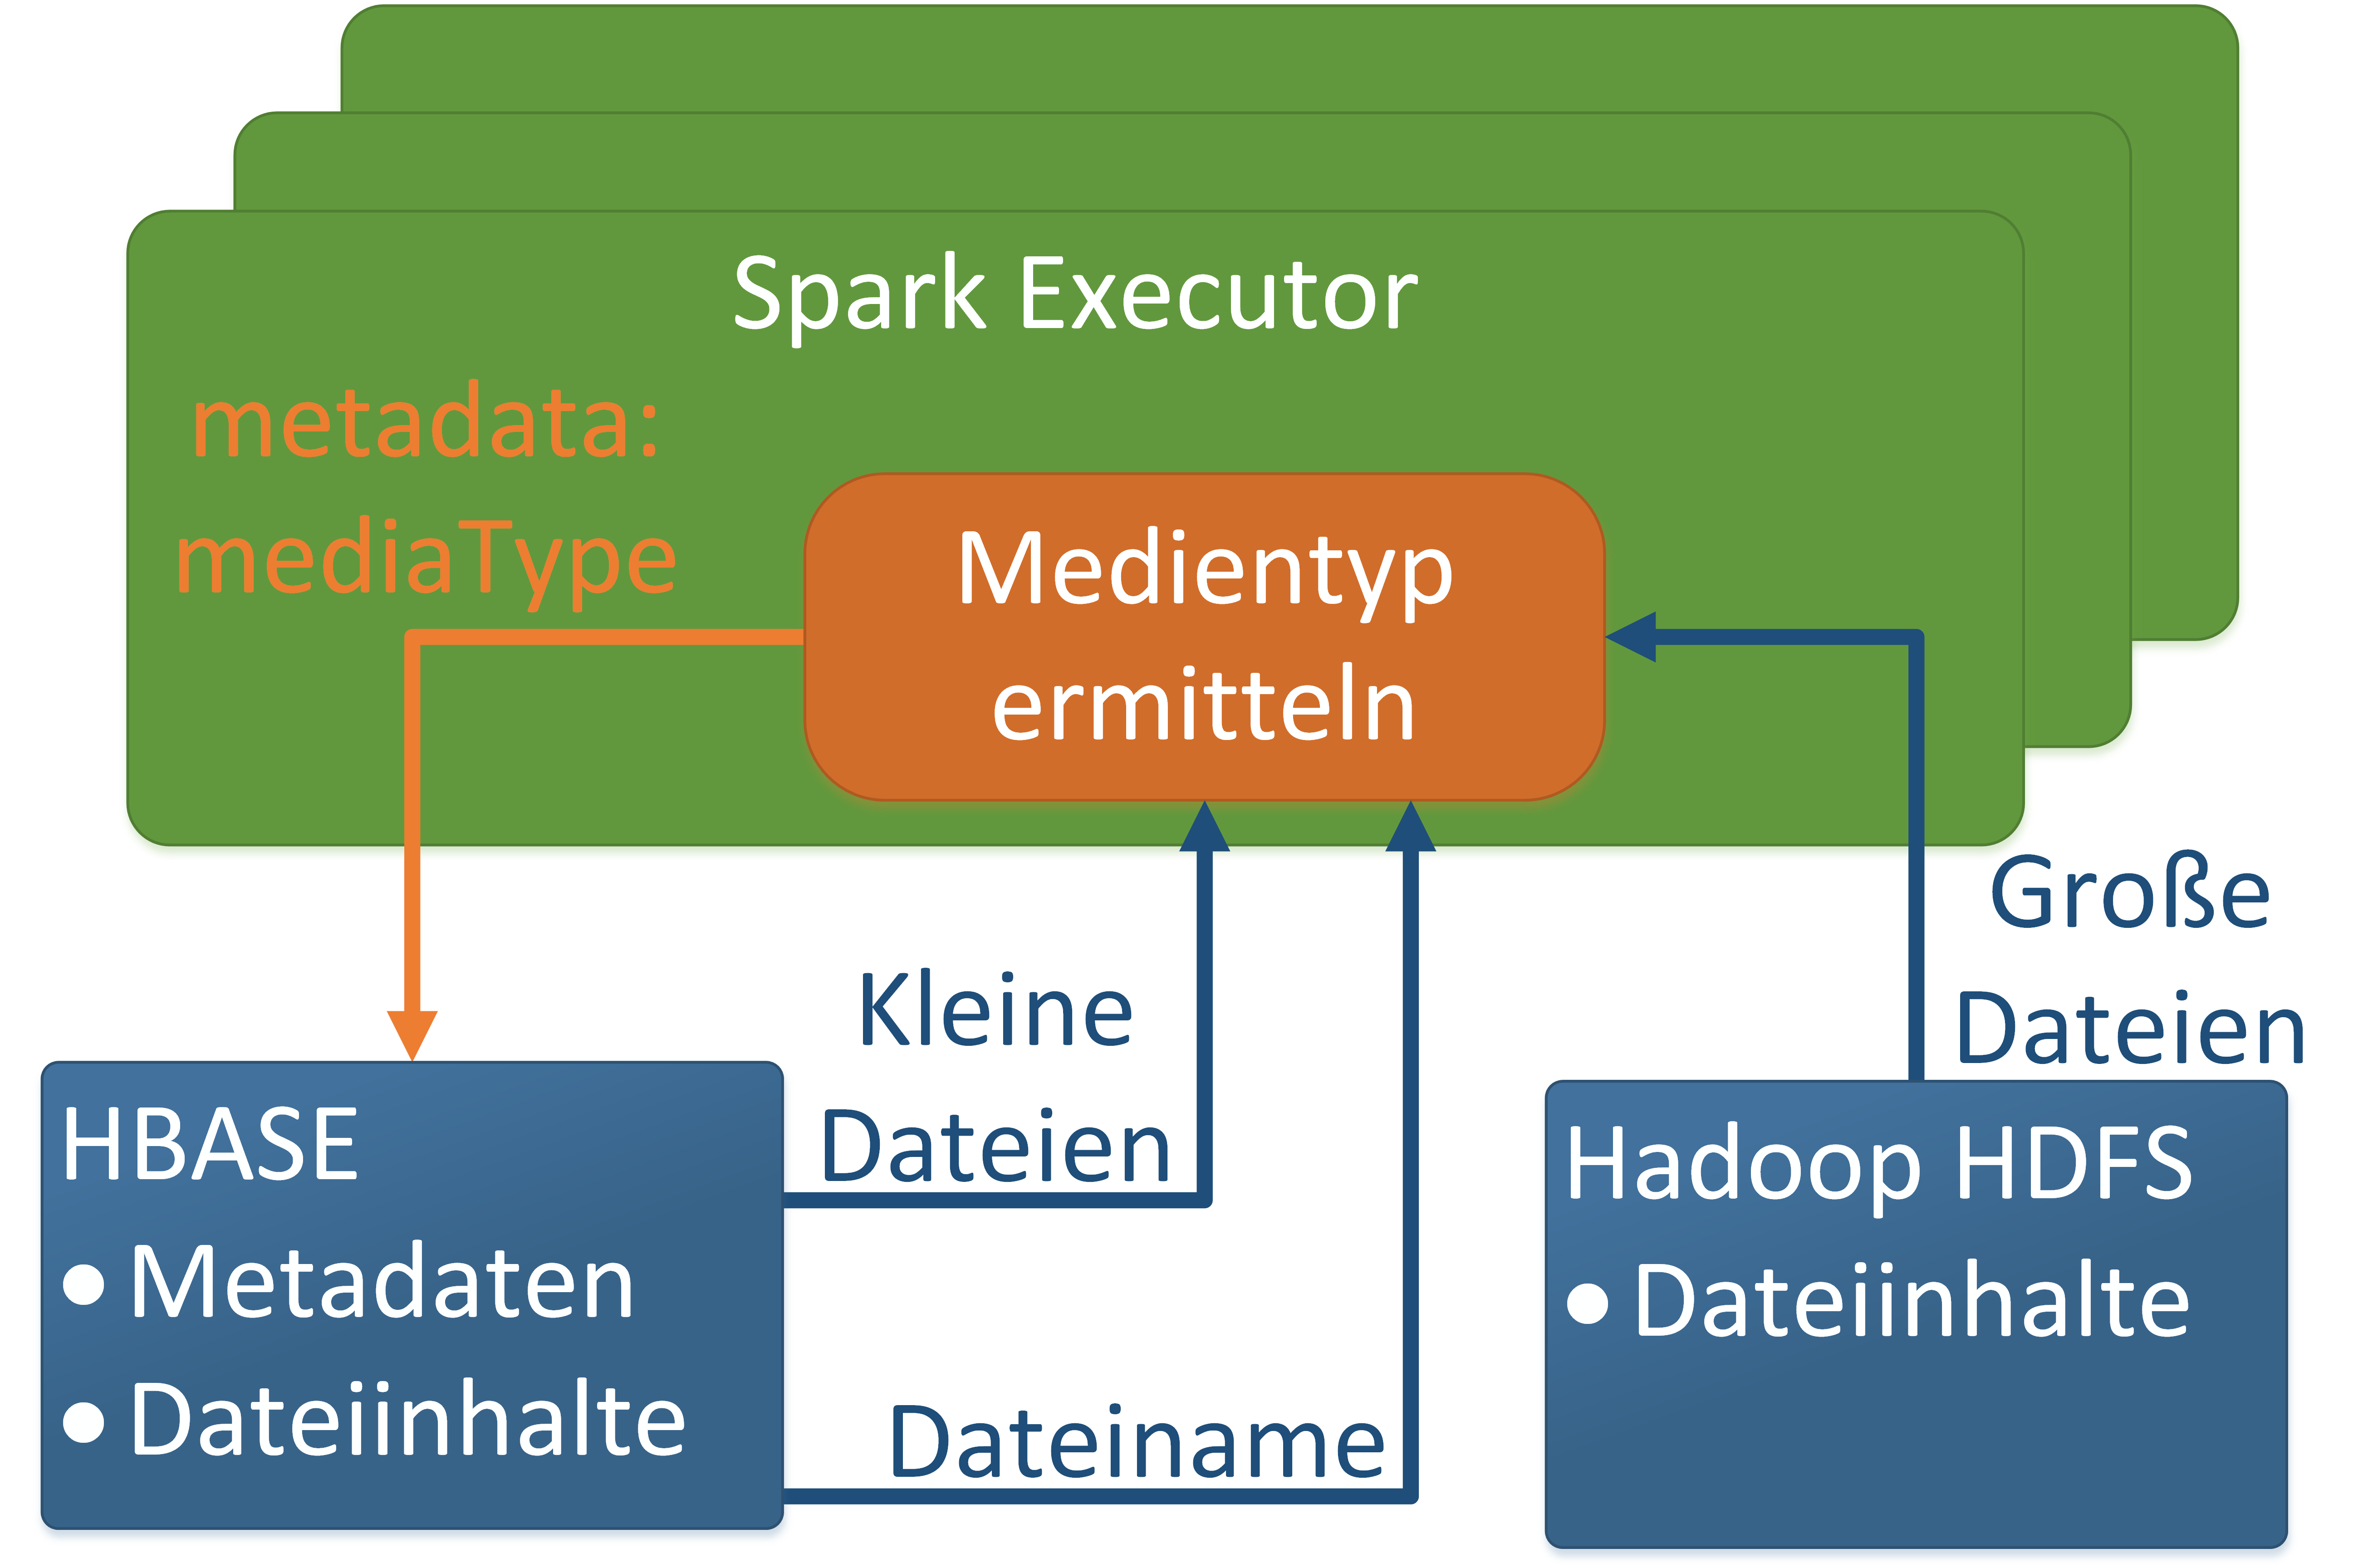
\includegraphics[width=0.78\textwidth]{./resource/spark_processing_media_types.png}
  \caption{Datenfluss bei der Ermittlung von Medientypen}
  \label{fig:data_processing_media_types}
\end{figure}

\noindent
Prinzipiell kann Apache Tika den Medientyp auch nur anhand der Dateiendung oder anhand des Dateiinhalts erkennen. Wird allerdings nur die Dateiendung angegeben, so könnten beispielsweise Bilddateien mit gefälschter Dateiendung nicht korrekt erkannt werden. Wird hingegen nur der Dateiinhalt angegeben, so prüft Tika formatspezifische Bytesequenzen, welche oftmals am Dateianfang stehen. Bei Textdateien hingegen kann es nur identifizieren, dass es sich um eine Textdatei handeln könnte. Gerade bei Textdateien ist es sinnvoll, die Dateiendung in die Analyse mit aufzunehmen, um ein genaueres Ergebnis zu erhalten. Dadurch kann Tika beispielsweise ermitteln, ob es sich um eine \acrshort{csv}-Datei oder eine \acrshort{html}-Datei handelt. Allerdings sollten diese Ergebnisse kritisch hinterfragt werden. Wie bereits erwähnt, könnte eine gefälschte Dateiendung bei Textdateien zu einem falschen Ergebnis führen.\\
Das Ermitteln der Medientypen ist gerade bei der Datenvisualisierung sinnvoll, da damit nach allen vorhandenen Bildern oder Videos gesucht werden kann.\footnote{Siehe auch Kapitel \ref{ch:data_visualization}.}

\subsection{Volltextsuche und Datenindexierung}
\label{subsec:file_indexing}
Um auf die Daten in der forensischen Analyseplattform einfach zugreifen zu können, wäre eine Volltextsuche sinnvoll. Diese sollte performant arbeiten, damit Ergebnisse zu Suchanfragen von beliebigen Schlüsselwörtern in Realzeit angezeigt werden können. Um dies zu ermöglichen, können die Dateiinhalte und Metadaten indexiert werden.\\

\noindent 
Es gibt hierzu zwei mögliche Open-Source Projekte, die eine Datenindexierung anbieten. Dies sind \textit{Apache Solr\texttrademark} und Elasticsearch\texttrademark. Beide bieten eine Indexierung auf Basis von Apache Lucene an. Apache Solr und Apache Lucene werden im Grundlagenkapitel \ref{sec:theory_solr} beschrieben. Solr und Elasticsearch bieten einen ähnlichen Funktionsumfang. Im Rahmen dieser Thesis wird jedoch Apache Solr aus nachfolgenden Gründen genutzt.\\
Apache Solr bietet einen Cloud-Modus an und nutzt Apache Zookeeper, um die einzelnen Instanzen zu koordinieren. Für Apache Solr existiert bereits eine Integration in das Hadoop-Framework und die hier verwendete \textit{Hortonworks Data Platform}.\footnote{Siehe Link: \url{https://docs.hortonworks.com/HDPDocuments/HDPS/HDPS-3.0.0/bk_solr-search-installation/content/ch_hdp-search.html}. Letzter Stand: 9.9.2018.}\\
Elasticsearch ist auch horizontal skalierbar und kann auf einem Computer-Cluster installiert werden. Allerdings wird ein eigener Mechanismus zur Koordination des Verbunds genutzt und es existiert für die \textit{Hortonworks Data Platform} kein Installationspaket zur Nutzung von Elasticsearch im Hadoop-Umfeld. Dies bedeutet, dass Elasticsearch eigenständig im Computer-Cluster ausgerollt und überwacht werden muss.\\

\noindent
Ein weiterer Punkt ist die Absicherung der Cluster mithilfe von Kerberos. Prinzipiell können beide Projekte mit Kerberos abgesichert werden. Allerdings ist die Funktionalität bei Elasticsearch nur in einem kostenpflichtigen Zusatzpaket der Firma \textit{Elastic}\footnote{Siehe Link: \url{https://www.elastic.co/}. Letzter Stand: 9.9.2018.} enthalten.\\

\noindent
Zuletzt unterscheiden sich beide Projekte auch in der Art und Weise, wie die Daten verteilt indexiert werden können. Bei Elasticsearch gibt es eine Bibliothek, welche die bereits bekannten \textit{Apache Spark Resilient Distributed Datasets} (RDDs) direkt in Elasticsearch indexieren kann.\footnote{Siehe Link: \url{https://www.elastic.co/guide/en/elasticsearch/hadoop/current/spark.html}. Letzter Stand: 9.9.2018.} Diese Möglichkeit eignet sich sehr gut, um Daten indexieren zu können.\\
Apache Solr hingegen bietet auch eine Möglichkeit mit Apache Spark Daten in die Solr-Cloud zu indexieren.\footnote{Siehe Link: \url{https://github.com/lucidworks/spark-solr}. Letzter Stand: 9.9.2018} Allerdings ist die Schnittstelle etwas umständlicher nutzbar, da keine RDDs sondern die bereits beschriebenen \textit{DateFrames} genutzt werden müssen.\\
%TODO Spark-Connector von Databricks?

\noindent
Ein weiterer Vorteil von Apache Solr ist die sogenannte \textit{\gls{solrcell}}, welche unter anderem auch Apache Tika nutzt, um Text aus PDF-Dokumenten, Word-Dokumenten oder Bildern zu extrahieren.\footnote{Siehe Link: \url{https://lucene.apache.org/solr/guide/7_4/uploading-data-with-solr-cell-using-apache-tika.html\#uploading-data-with-solr-cell-using-apache-tika}. Letzter Stand: 11.9.2018.} Diese Funktionalität könnte gegebenenfalls wiederverwendet werden, um beliebige Dateiinhalte automatisch zu indexieren. Eine ähnliche Funktionalität bei Elasticsearch müsste selbst implementiert werden.\\

\noindent
Eine interessante Möglichkeit Dateien in Solr zu indexieren, bietet das Open-Source Projekt \textit{Lily HBase Indexer}.\footnote{Siehe Link: \url{https://github.com/NGDATA/hbase-indexer}. Letzter Stand: 9.9.2018.} Damit können Daten direkt aus HBASE in den Solr-Cluster indexiert werden. 
Im Rahmen der Thesis wird letzteres Projekt genutzt, um die Metadaten aus HBASE in Solr zu indexieren. Abbildung \ref{fig:hbase_solr_indexing} stellt die physikalische Aufteilung mit dem Lily HBase Indexer dar.\\
\begin{figure}[ht]
  \centering
  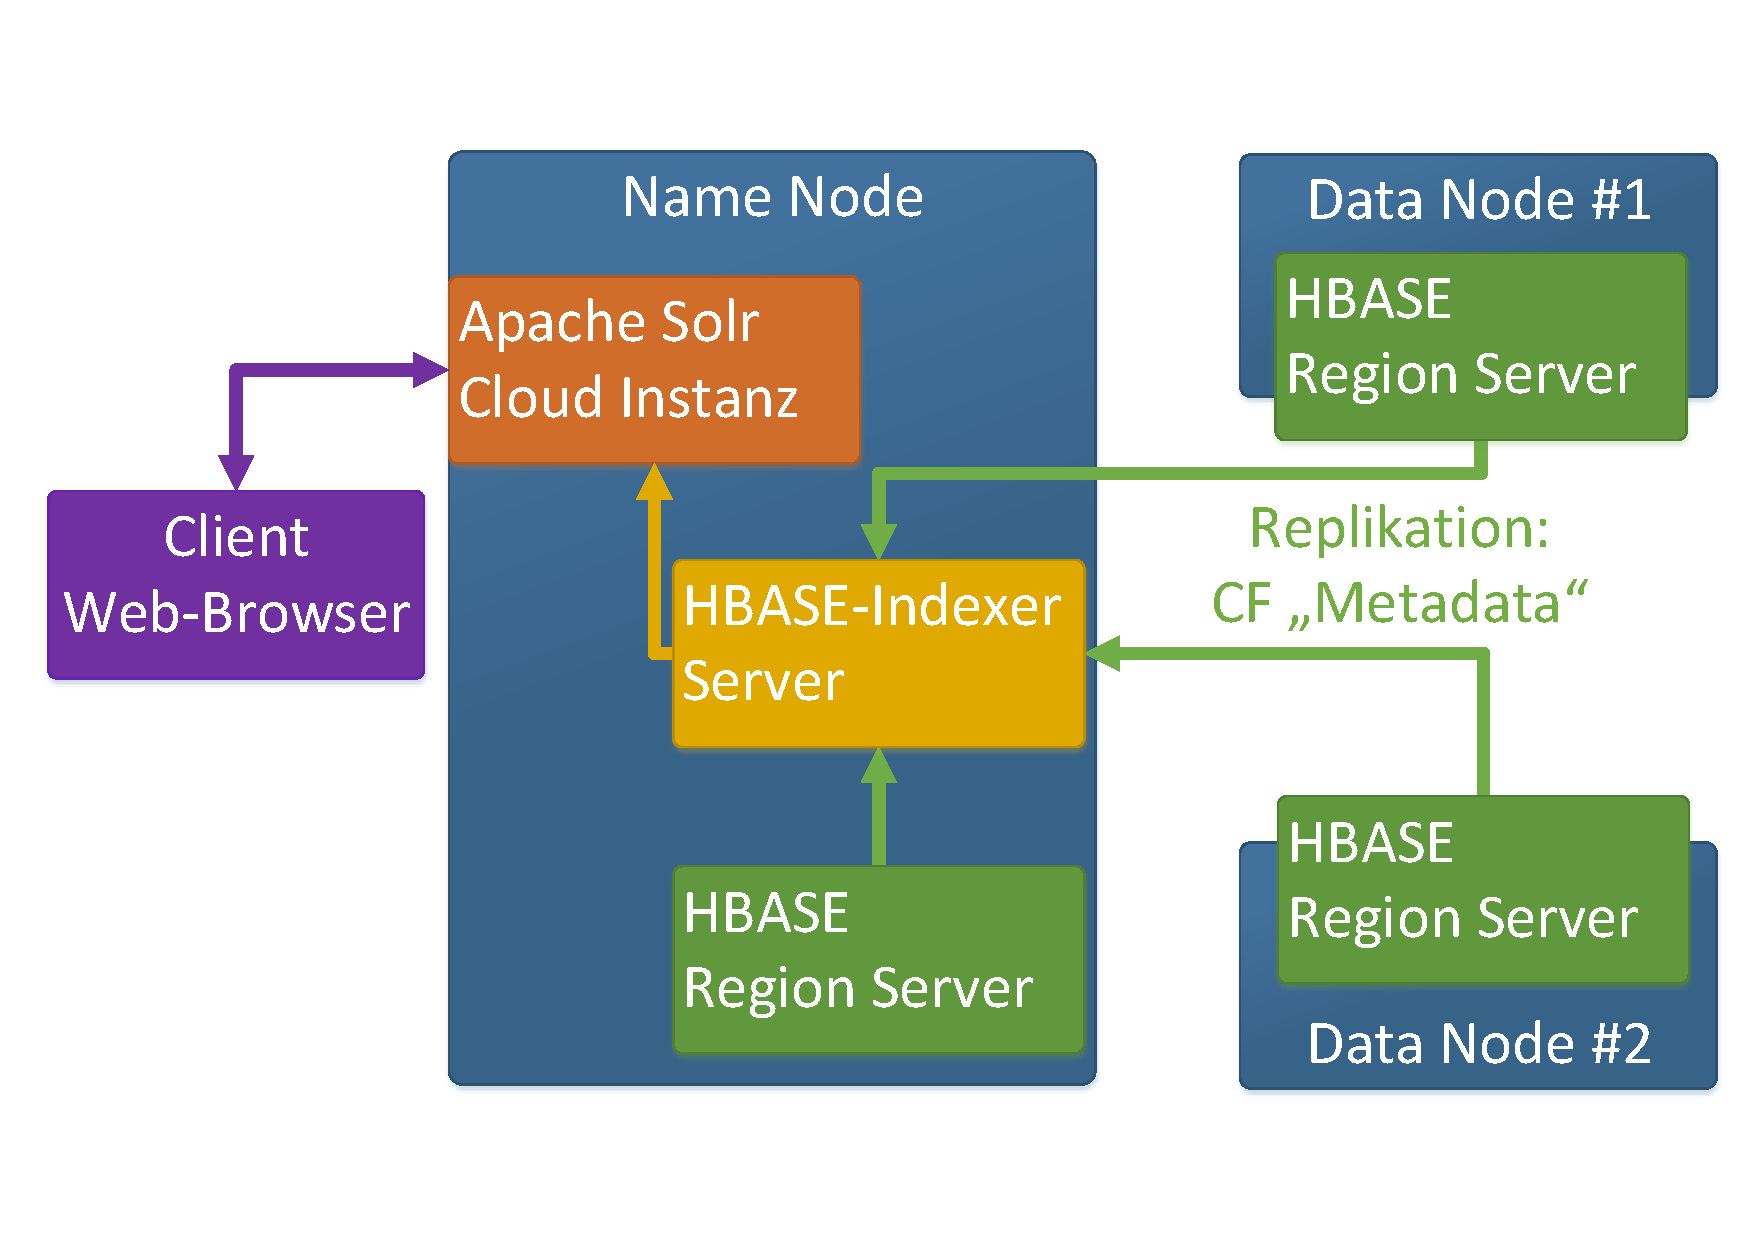
\includegraphics[width=\textwidth]{./resource/hbase_solr_indexierung.pdf}
  \caption{Indexierung von Daten aus HBASE in Solr}
  \label{fig:hbase_solr_indexing}
\end{figure}

\noindent
Das Projekt selbst bietet mehrere Möglichkeiten, wie Daten indexiert werden können. Die hier genutzt Variante basiert auf einem sogenannten \textit{Side-Effect Processor}.\cite{hbase_sep} 
Dieser Side-Effect Processor registriert sich bei HBASE als weiterer Knoten zur Datenreplikation. Aus Sicht von HBASE werden die Daten zu einem weiteren Knoten repliziert. Die Replikation läuft asynchron im Hintergrund und soll dadurch die Schreibgeschwindigkeit bei HBASE nicht beeinflussen. Jede neue Zeile und jede Datenmodifikation in HBASE wird automatisch repliziert und dadurch in Solr indexiert.
Auch das Löschen von Zeilen wird entsprechend in Solr übernommen. Damit HBASE die Daten repliziert, müssen die Tabellen und deren Spaltenfamilien extra zur Replikation markiert werden. Unabhängig von dieser Replikation, werden die Daten immer auf mehreren Knoten repliziert, da HBASE die Informationen in Dateien auf dem HDFS ablegt. Und jede Datei im HDFS wird mindestens dreifach repliziert.\\

\noindent
Ein Nachteil an dieser Variante ist die Tatsache, dass keine Binärdaten mithilfe von \textit{Solr Cell} verteilt indexiert werden können. Hierzu müsste das \textit{Lily Hbase Indexer}-Projekt erweitert werden.\\
Ein weiteres Hindernis zeigt sich bei der Software-Installation. So kann zwar Apache Solr für das Computer-Cluster nachinstalliert werden. Allerdings wird Solr nur auf einem Knoten installiert. An dieser Stelle konnte noch Möglichkeit gefunden werden, wie Solr auf allen Knoten im Cluster ausgerollt werden kann. Dies sollte jedoch technisch möglich sein.\\
Für den Lily Hbase Indexer wird eine eigene kleine Server-Komponente benötigt, welche eigentlich auf allen Knoten installiert sein müsste, damit die Daten nach dem Prinzip der Datenlokalität ordnungsgemäß indexiert werden können. Auch diese Server-Komponente läuft derzeit nur auf einem Knoten.\\
Darüber hinaus wird der Lily Hbase Indexer derzeit nicht weiterentwickelt\footnote{Die letzte Änderung im Git-Repository erfolgte im Dezember 2016.}. In einigen Tests war die Integration des Indexers nur mit HBASE in der Version 1.X.X möglich. Eine erfolgreiche Integration mit bereits verfügbaren neueren Versionen von HBASE  (ab Version 2.X.X) war nicht möglich.\\ 

\noindent
Somit wäre es sinnvoll einen neuen Ansatz zu finden, oder den bisherigen Indexer selbst weiterzuentwickeln. An dieser Stelle sollte das \textit{Spark-Solr} Projekt nochmals näher betrachtet werden.\footnote{Siehe Link: \url{https://github.com/lucidworks/spark-solr}. Letzter Stand: 9.9.2018} Diese Implementierung könnte eventuell die bestehenden Probleme lösen. 



\section{Praxisbeispiele und deren Optimierungen}
Bei der Verarbeitung großer Datenmengen sollte immer das Prinzip der Datenlokalität berücksichtigt werden. Darüber hinaus gibt es weitere Optimierungen, um die Datenmenge auf das nötige Minimum zu reduzieren und die verfügbaren Ressourcen optimal auszunutzen. Im Hadoop-Umfeld und bei der Entwicklung mit Apache Spark ist es besonders wichtig zu verstehen, auf welchen Knoten welche Teile des Programmcodes ausgeführt werden. Der Entwickler sollte immer wissen, in welchem Verarbeitungskontext er sich befindet. Zu dieser Problematik werden in diesem Kapitel einige Beispiele herausgegriffen, welche während der Bearbeitung dieser Thesis aufgetreten sind.\\

\subsection*{Datenminimierung}
Wie bereits beschrieben können die Metadaten aus HBASE mithilfe des \textit{HBASE-Spark Connectors} geladen werden. Hierbei können die einzelnen Zeilen mit allen Spalten geladen und in Spark verarbeitet werden. In Spark wiederum können diese \textit{RDDs} nach bestimmten Kriterien gefiltert werden. Beispielsweise werden bei der Berechnung von Hashsummen die Zeilen nach logischen Dateien gefiltert. Verzeichnisse oder symbolische Links werden verworfen. Zusätzlich wird für die Berechnung von Hashsummen auch nur der Dateiinhalt benötigt. Andere Metadaten sind überflüssig. Auch diese Werte können in den Spark RDDs einfach herausgefiltert werden. Allerdings befinden sich diese Daten zu dem Zeitpunkt schon in den einzelnen Spark Executoren. Viel effizienter ist es, diese Filterungen schon bei der Anfrage in der Datenbank durchzuführen. So bietet der \textit{HBASE-Spark Connector} die Möglichkeit diverse Filter auf Zeilen und Spalten anzuwenden, um bereits in den einzelnen RegionServer die benötigte Datenmenge auf das notwendige Minimum zu begrenzen. Diese Optimierung fällt bei kleinen Datenmengen in einer Testumgebung kaum ins Gewicht. Bei großen Datenmengen in einem produktiven Cluster, kann hier aber einiges an Ressourcenverbrauch und Zeit eingespart werden, wenn die Datenmenge schon direkt in HBASE gefiltert wird.\\

\subsection*{Lazy Loading}
Ein weiterer Aspekt, um den Ressourcenverbrauch minimal zu halten, ist das sogenannte \textit{Lazy Loading}. Beim diesem Entwurfsmuster aus der Softwareentwicklung geht es darum, die Daten nur dann zu laden und zu verarbeiten, wenn sie auch wirklich benötigt werden. Apache Spark implementiert dieses Entwurfsmuster in den Spark RDDs.\cite{spark_rdd}\\
Listing \ref{lst:spark_lazy_loading} zeigt ein Beispiel. Dabei werden die Methoden unterteilt in \textit{Transformationen}, wie beispielsweise \textit{map()} oder \textit{filter()} und \textit{Aktionen}, wie zum Beispiel \textit{first()} oder \textit{reduce()}. Alle Transformationen sind \textit{lazy}. Wenn nun eine Transformation auf einem RDD aufgerufen wird, so wird diese Methode noch nicht ausgeführt. Sie wird erst ausgeführt sobald auf dem RDD auch eine Aktion ausgeführt wird. Dies kann die Effizienz der Datenausführung steigern, da die Daten auch nur verarbeitet werden, wenn ein Ergebnis einer Aktion benötigt wird.

\begin{lstlisting}[label={lst:spark_lazy_loading},caption= Lazy Loading bei Apache Spark ,captionpos=b,frame=single,style=customjava]
JavaRDD<Data> data = getData();
// Definiere Transformationen
data.map(x -> convert(x))
	.filter(Objects::nonNull)
	.map(y -> convertToZ(y))
	// Erst nachdem die "Aktion" first() aufgerufen wird,
	// werden auch die Daten geladen und verarbeitet.
	.first()
\end{lstlisting}

\subsection*{Zwischenergebnisse Speichern}
Wie bereits erläutert unterscheidet Apache Spark bei den Methoden zwischen Transformationen und Aktionen, die auf ein RDD angewendet werden. Meistens werden ein oder mehrere Transformationen auf ein RDD angewendet und zum Schluss folgt eine Aktion, welche das Ergebnis der Datenverarbeitung zurückliefert. In vielen Fällen werden mehrere Ergebnisse berechnet, welche teilweise auf ähnlichen Transformationen aufbauen. Allerdings kann ein RDD, welches durch eine abschließende Aktion einmal ausgeführt wurde, nicht einfach wiederverwendet werden. Spark bietet aber die Möglichkeit Zwischenergebnisse einzelner RDDs explizit zwischenzuspeichern, um sie für die Berechnung anderer Ergebnisse wiederzuverwenden. Ein Beispiel aus dem forensischen Umfeld ist die Berechnung von Hashsummen. Beispielsweise sollen die Hashsummen von allen Dateien berechnet werden und gespeichert werden. Zusätzlich sollen Duplikate (Dateien mit gleicher Hashsumme) ausgegeben werden. Das sind zwei unterschiedliche Ergebnismengen, wobei die Ermittlung der Duplikate auf der Berechnung der Hashsummen aufbaut. Prinzipiell müssten jetzt zwei unabhängige RDDs erstellt werden. Wobei beide im ersten Schritt die Hashsummen der Rohdaten berechnen. Diese Arbeit wird bei zwei unabhängigen RDDs im Computer-Cluster auch zweifach ausgeführt und benötigt auch doppelt so viele Ressourcen. Daher wäre es in diesem Beispiel sinnvoll, die Berechnung der Hashsummen zwischenzuspeichern und die Ermittlung von Dateiduplikaten darauf aufzubauen.\\
Diese Zwischenspeicherung spart Ressourcen und erhöht die Performanz der Datenverarbeitung. Hierbei ist es bei Spark möglich, die Daten im Arbeitsspeicher zwischenzuspeichern oder falls der Speicher nicht ausreicht, auf einen persistenten Datenspeicher auszuweichen. Allerdings müssen die Daten serialisierbar sein. Dies ist nicht immer gegeben. Letztlich ist das Zwischenspeichern von Daten (Caching) in Spark eine wichtige Funktion, um die Geschwindigkeit der Datenverarbeitung zu erhöhen.\cite{spark_rdd}

\subsection*{Verteilte Datenverarbeitung}
%Balancing and Repartitionieren. Aufteilung der Last zu gleichen Teilen!
Bei der lokalen Entwicklung von Spark-Anwendung ist es einfach, die Resultate eines RDDs über eine Konsole auszugeben. Dadurch kann schnell geprüft werden, ob die Ergebnisse aus fachlicher Sicht korrekt sind. Was hingegen auf kleinen lokalen Testknoten nicht geprüft werden kann, ist die korrekte Skalierung bei großen Datenmengen. Hierbei muss genau überlegt werden, wie die Ergebnisse ausgegeben werden sollen (siehe Listing \ref{lst:spark_rdd_collect}). 

\begin{lstlisting}[label={lst:spark_rdd_collect},caption= Anzeige der Ergebnisse eines Spark RDDs ,captionpos=b,frame=single,style=customjava]

HbaseReader hbr = new HbaseReader(jsc, hbaseConfigFile);
JavaRDD<Metadata> forensicMetadata = hbr.getForensicMetadata();

// collect()-Methode
forensicMetadata.collect().stream()
	.forEach(m -> LOGGER.info("Entry = .", m));

// take(int amount)-Methode	
forensicMetadata.take(10).stream()
	.forEach(m -> LOGGER.info("Entry = .", m));	
\end{lstlisting}

\noindent
In der ersten Variante wird auf dem RDD die Methode collect() aufgerufen und die daraus erhaltene Liste von Objekten wird über ein Logger-Objekt in das Log-File dieser Ausführung geschrieben.\\
Auf der ersten Blick ist aber nicht ersichtlich, was diese Methode wirklich bewirkt. Wie bereits in Kapitel \ref{sec:theory_spark} beschrieben, wird bei der Ausführung einer Spark-Anwendung ein sogenannter Spark-Driver gestartet. Dieser wiederum fordert eine gewisse Anzahl von Executoren an, welche die eigentliche Datenverarbeitung übernehmen (Master-Slave-Prinzip). Die Executoren arbeiten auf einzelnen Knoten innerhalb des Clusters. Ein Spark RDD wird bei der Verarbeitung auf diese Executoren aufgeteilt. Doch je nachdem, welche \textit{Aktion} die Ergebnismenge des RDDs zurückliefert, wird das Ergebnis weiterhin verteilt gespeichert oder aber es wird an den Spark-Driver zurückgesendet. In dem Moment, in welchem beispielsweise die collect()-Methode auf einem RDD ausgeführt wird, werden die Daten des RDDs \textit{eingesammelt}. Dies bedeutet, dass die Daten des RDDs, welche vorher verteilt auf allen Executoren im Arbeitsspeicher geladen wurden, nun jetzt an den Spark-Driver geschickt werden. Dieser Mechanismus ist für sich genommen nicht problematisch und funktioniert auch gerade beim Testen mit kleinen Datenmengen. Bei großen RDDs werden auch alle Ergebnisse an den Driver geschickt. Da der Driver aber nur begrenzte Ressourcen zugeteilt bekommt, wird in den meisten Fällen der Arbeitsspeicher ausgehen und die Anwendung wird abgebrochen.\\

\noindent
Daher ist es auch schon beim Testen mit kleinen RDDs sinnvoll, die Daten entweder verteilt auszugeben oder die Ergebnismenge, welche an Driver gesendet wird, zu begrenzen. Im zweiten Teil von Listing \ref{lst:spark_rdd_collect}  wird hierzu die take()-Methode verwendet. Diese verhält sich wie  die collect()-Methode mit dem Zusatz, dass sie nur eine bestimmte Anzahl von Einträgen einsammelt. Dadurch wird selbst bei größeren RDDs der Speicher nicht ausgehen.\\
In der finalen Lösung sollten die Ergebnisse auch verteilt gespeichert werden.  So können mithilfe der Methode \textit{saveAsTextFile()} die Ergebnisse eines Spark RDDs in das HDFS gespeichert werden. Hierbei legt jeder Executor eine eigene Textdatei im HDFS an und speichert dort seinen Anteil der Ergebnismenge. Dadurch ist eine korrekte verteilte Datenverarbeitung auch bei großen Datenmengen ohne Ressourcenengpass möglich. 


\section{Leistungsanalyse}
\label{sec:performance_analysis}
Die hier entwickelte forensische Analyseplattform soll den Forensiker dabei unterstützen, die Daten schnell verarbeiten und analysieren zu können. Hierbei spielt gerade die Zeitdauer zur Datenanalyse ein wichtige Rolle. In diesem Kapitel soll daher getestet werden, wie lange die Datenaufbereitung dauert. Einerseits soll ermittelt werden, wie lange es dauert bis ein großes Datenträgerabbild in die Analyseplattform importiert wurde und andererseits soll die Dauer der Datenverarbeitung getestet werden. Wobei die eigentliche Datenverarbeitung aus der Berechnung der Hashsummen und der Ermittlung der Medientypen besteht.\\

\noindent
Da im Hadoop-Cluster mehrere Knoten im Verbund arbeiten und unterschiedliche Technologien eingesetzt werden, ist es sehr schwer zuverlässige Testszenarien durchzuführen. Daher sollten die Ergebnisse dieser Testreihe vielmehr Anhaltspunkte liefern, in welchem groben Zeitraum wie viele Daten verarbeitet werden können.\\

\noindent
Das hier genutzte Testcluster besteht aus 3 Knoten und bildet daher das kleinste mögliche Hadoop-Cluster mit der standardmäßigen dreifachen Datenreplikation. Die drei Knoten sind identisch und enthalten jeweils eine Intel Core i5-6500 Quad-Core CPU ohne Hyperthreading, 32 GB Arbeitsspeicher, eine 512 GB SSD und eine 2 TB große Magnetfestplatte. Als Betriebssystem wird CentOS 7 (Version 7.5.1804) genutzt. Darauf ist die Hortonworks Data Platform in der Version 2.6.5 installiert. Während das Betriebssystem jeweils auf der SSD installiert ist, werden die Daten aus dem HDFS auf den langsameren und größeren Magnetfestplatten gespeichert. Dadurch hat das HDFS eine maximal Gesamtkapazität von knapp 6 TB. Die Knoten kommunizieren untereinander in einem getrennten Netzwerk über Gigabit-Ethernet.\\  

\noindent
Tabelle \ref{tab:performance_results} zeigt die Zeitdauer des Importvorgangs und der Datenverarbeitung. Das erste Datenträgerabbild ist knapp 10 GB groß und enthält eine Ubuntu Installation. Das zweite Datenträgerabbild ist ungefähr 155 GB groß und enthält eine Windows 10 Installation. Beide Datenträger wurden im Rahmen dieser Thesis erstellt und werden jeweils vier Mal in das Analysesystem importiert und verarbeitet.\footnote{Siehe Kapitel \ref{testdatacreation}.} \\


\begin{table}[ht]
\centering
\begin{tabular}{l|l|l}
Datenträgerabbild & Dauer des Datenimports & Dauer der Datenverarbeitung	\\ \hline
Ubuntu Image \#1 		& 9 min 45 sec	& 4 min 42 sec  \\
Ubuntu Image \#2 		& 7 min 38 sec	& 4 min 50 sec  \\
Ubuntu Image \#3 		& 7 min 55 sec	& 4 min 45 sec  \\
Ubuntu Image \#4 		& 9 min 30 sec	& 4 min 43 sec	\\ \hline
Windows Image \#1 		& 4 h 32 min		& 35 min 26 sec	\\
Windows Image \#2 		& 4 h 37 min		& 28 min 12 sec	\\
Windows Image \#3 		& 4 h 26 min		& 29 min 40 sec	\\
Windows Image \#4 		& 4 h 43 min		& 30 min 06 sec	\\
\end{tabular}
\caption{Zeitdauer der Datenverarbeitung}
\label{tab:performance_results}
\end{table}

\noindent
Aus den Ergebnissen ist ersichtlich, dass gerade der Datenimport sehr viel Zeit benötigt, da alle Dateien aus dem Datenträgerabbild vollständig in das Hadoop-Cluster importiert und gespeichert werden müssen. Interessanterweise ist das Hadoop-Cluster nicht einmal annähernd voll ausgelastet. Über die Monitoring-Oberfläche des Hadoop-Clusters zeigt sich, dass die CPU- und Speicher-Auslastung nicht sonderlich hoch ist. Allerdings ist die Schreibrate von HBASE sehr niedrig. An dieser Stelle besteht ein deutlicher Optimierungsbedarf, um eine höhere Performanz bei HBASE zu erzielen. Denn wenn schon mehr als vier Stunden nur für das Importieren eines 155 GB großen Datenträgers benötigt werden, dann ist es aus Anwendersicht deutlich schneller den Datenträger mit Autopsy zu analysieren.\\
Bisher konnte noch nicht abschließend geklärt werden, weshalb die Datenspeicherung in HBASE so langsam ist. Es könnte an einer Fehlkonfiguration im Cluster liegen, oder an einer falschen Dimensionierung der verwendeten Ressourcen von HBASE. Es könnte auch an der Datenimport-Anwendung liegen, falls diese das Hochladen der Daten nicht optimal parallelisiert.\\

\noindent
Die Geschwindigkeit beim Datenimport ist auch abhängig von den genutzten Festplatten. Das HDFS im Testcluster ist so konfiguriert, dass die Daten auf die langsameren magnetischen Festplatten mit 7200 Umdrehungen pro Minute geschrieben werden. 
Hier könnte die Performanz des Clusters noch erhöht werden, wenn SSDs die Daten im HDFS speichern würden. Allerdings ist dieser Ansatz aus Kostengründen nicht immer realisierbar.\\

\noindent
Der Datendurchsatz könnte gegebenenfalls auch erhöht werden, wenn mehrere Datenträger parallel in das Analysesystem importiert werden. 
Somit könnte eine optimale Auslastung der Hadoop-Komponenten erreicht werden. Zumal bei forensischen Analysen oftmals mehrere Asservate sichergestellt werden und diese dann auch parallel verarbeitet werden sollen.\\

\noindent
Andererseits macht es aus Anwendersicht keinen Sinn, zuerst das Asservat vollständig zu importieren und erst danach mit der Aufbereitung und Analyse zu beginnen. Die Daten können mit Spark auch schon verarbeitet werden, sobald die ersten Dateien im HDFS oder in HBASE gespeichert werden. Durch diesen \textit{Streaming-Modus} hätte der Nutzer schon während dem Import die Möglichkeit, die ersten eingehenden Daten zu analysieren. Er müsste nicht warten bis der Import vollständig beendet ist. Auch die Datenindexierung könnte schon während dem Importvorgang durchgeführt werden. Dieser Ansatz wäre sinnvoll, um die Verarbeitungszeit nochmals deutlich zu senken und die Verarbeitungsschritte besser parallelisieren zu können.\\
In einer zukünftigen Weiterentwicklung sollte daher der Datenimport und die Verarbeitung dahingehend überarbeitet werden.